\documentclass[12pt]{article}
\usepackage{amsfonts, amssymb, amsmath, amsthm}
\usepackage[margin=1in]{geometry}
\usepackage{tikz}
\usepackage{pgfplots}
\pgfplotsset{compat=1.18}

\title{Explainer: Problem 4 (Rudin 7.10) --- Fractional Part Series}
\author{}
\date{}

\begin{document}
\maketitle

\section*{What's going on?}
The function is $f(x) = \sum_{n=1}^{\infty} \frac{(nx)}{n^2}$, where $(t) = t - [t]$ is the \textbf{fractional part} of $t$.

\begin{center}
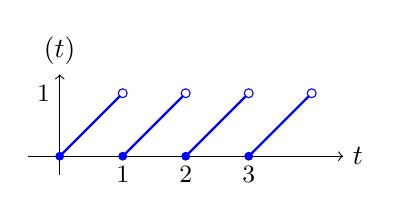
\begin{tikzpicture}[scale=0.8]
    \draw[->] (-0.5,0) -- (4.5,0) node[right] {$t$};
    \draw[->] (0,-0.3) -- (0,1.3) node[above] {$(t)$};
    \foreach \k in {0,1,2,3} {
        \draw[thick, blue] (\k,0) -- (\k+1,1);
        \fill[blue] (\k,0) circle (2pt);
        \draw[blue] (\k+1,1) circle (2pt);
        \fill[white] (\k+1,1) circle (1.5pt);
    }
    \node[below] at (1,0) {\small $1$};
    \node[below] at (2,0) {\small $2$};
    \node[below] at (3,0) {\small $3$};
    \node[left] at (0,1) {\small $1$};
\end{tikzpicture}
\end{center}

The fractional part $(t)$ is a sawtooth wave: it climbs linearly from $0$ to $1$, then jumps back to $0$ at every integer. It's continuous except at integers, where it has a jump discontinuity.

\section*{Where is $(nx)$ discontinuous?}

The function $t \mapsto (t)$ is discontinuous at integers. So $x \mapsto (nx)$ is discontinuous when $nx$ is an integer, i.e.\ when $x$ is a rational of the form $\frac{k}{n}$.

The $n$th term $\frac{(nx)}{n^2}$ is discontinuous at $x = \frac{k}{n}$ for $k \in \mathbb{Z}$.

\section*{Where is $f$ discontinuous?}

\textbf{At every rational $x = p/q$:} The term with $n = q$ (and multiples of $q$) is discontinuous there.

\textbf{At irrationals:} Every single term $(nx)/n^2$ is continuous (since $nx$ is never an integer when $x$ is irrational). The series converges uniformly (by the $M$-test, since $|(nx)/n^2| \leq 1/n^2$ and $\sum 1/n^2 < \infty$), so the sum of continuous functions is continuous.

Wait --- but at rationals, the series also converges uniformly! So why isn't $f$ continuous at rationals?

\textbf{The subtlety:} At $x = p/q$, some of the terms themselves are discontinuous. Theorem 7.12 says ``uniform limit of continuous functions is continuous.'' If the individual terms aren't all continuous at $x_0$, the theorem doesn't apply.

\section*{Proving $f$ is actually discontinuous at rationals}

At $x = p/q$ (in lowest terms), the term $(qx)/q^2$ has a jump of size $1/q^2$ (since $(qt)$ jumps by $1$ when $t$ crosses $p/q$). You can show this jump survives in the sum $f$ by checking that the other terms are continuous there or that their jumps don't cancel.

\section*{The discontinuities form a countable dense set}

\textbf{Countable:} The rationals $\mathbb{Q}$ are countable.

\textbf{Dense:} $\mathbb{Q}$ is dense in $\mathbb{R}$.

\section*{Riemann integrability despite the discontinuities}

This is the beautiful part: $f$ is discontinuous on a countable dense set, yet still Riemann-integrable!

\textbf{Key tool:} The series converges uniformly (by the $M$-test with $M_n = 1/n^2$). Each partial sum $S_N(x) = \sum_{n=1}^N (nx)/n^2$ is a finite sum of bounded functions with finitely many discontinuities in any interval, hence each $S_N$ is Riemann-integrable. Theorem 7.16 says: the uniform limit of Riemann-integrable functions is Riemann-integrable.

\section*{Proof outline}
\begin{enumerate}
    \item \textbf{Uniform convergence:} $|(nx)/n^2| \leq 1/n^2$, Weierstrass $M$-test.
    \item \textbf{Discontinuities at rationals:} Show the jump from $(nx)$ at $x = p/q$ doesn't cancel.
    \item \textbf{Continuity at irrationals:} All terms continuous $+$ uniform convergence $\Rightarrow$ sum continuous (Thm 7.12).
    \item \textbf{Riemann-integrable:} Each $S_N \in \mathscr{R}$, uniform convergence, Thm 7.16.
\end{enumerate}

\end{document}